\section{Modello e addestramento}
\label{sec:method}

\subsection{Architettura}

Il modello è la U-Net della Sezione~\ref{sec:background} con un \textbf{encoder
ResNet18 pre-addestrato su ImageNet} (Figura~\ref{fig:architectures}): con meno di
500 osservazioni di training, imparare da zero bordi e texture spreca il budget di
dati. La testa di classificazione viene scartata e i quattro blocchi convoluzionali
alimentano il decoder U-Net attraverso le skip connection. Una riscrittura
algebrica una tantum ripiega lo stem RGB e la normalizzazione ImageNet in una
convoluzione a canale singolo esattamente equivalente, così le immagini in scala di
grigi entrano direttamente a un terzo della banda d'ingresso. L'architettura resta
poi fissa per tutto lo studio: una variabile per esperimento è ciò che rende
significativi i confronti.

Tre alternative sono state considerate e scartate per ragioni dichiarate e
verificabili. Le \textbf{architetture di instance segmentation} come Mask
R-CNN~\cite{maskrcnn} ricostruiscono ogni maschera da una griglia $28 \times 28$
dentro un box allineato agli assi -- un sovracampionamento di $\sim\!25\times$ per
oggetti la cui proprietà distintiva è essere larghi pochi pixel e lunghi centinaia
-- e filamenti allungati e diagonali producono box sovrapposti e quasi tutti di
sfondo, il regime peggiore per l'anchor matching. L'affermazione è stata poi
verificata empiricamente invece di restare sulla carta: un detector
YOLOv8x-seg~\cite{yolo} addestrato sullo stesso split raggiunge un punteggio a
istanze competitivo (PQ $0{,}426$) ma un Dice nettamente peggiore ($0{,}632$ contro
$0{,}68$), confermando la scelta per il punteggio della traccia. \textbf{Encoder più
grandi e transformer}: in ogni capacità e risoluzione provata la qualità delle
maschere accoppiate non si è mai mossa (Sezione~\ref{sec:error}), quindi la capacità
non è il vincolo attivo, mentre il budget di dati sconsiglia modelli più affamati.
Le \textbf{pipeline non neurali} (sogliatura più morfologia): il contrasto H-alpha
varia fortemente tra osservazioni, e una regola fotometrica globale non può
separare i filamenti da macchie solari e oscuramento al bordo.

\begin{figure}[t]
    \centering
    \begin{minipage}[c]{0.46\linewidth}
        \centering
        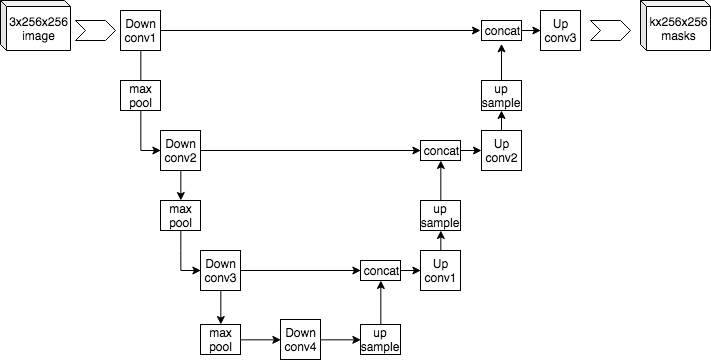
\includegraphics[width=\linewidth]{figures/unet_architecture.png}
    \end{minipage}\hfill
    \begin{minipage}[c]{0.50\linewidth}
        \centering
        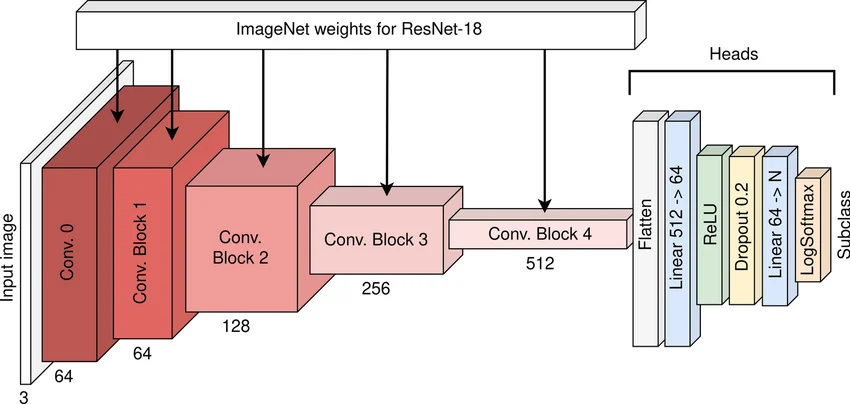
\includegraphics[width=\linewidth]{figures/resnet18_architecture.png}
    \end{minipage}
    \caption{A sinistra: l'encoder--decoder U-Net con le skip connection. A destra:
    l'encoder ResNet18 che sostituisce quello da zero; la testa di classificazione
    viene scartata e i quattro blocchi convoluzionali alimentano il decoder U-Net.}
    \label{fig:architectures}
\end{figure}

\subsection{Loss, ottimizzazione e implementazione}

La loss è una combinazione a pesi uguali di binary cross-entropy e soft
Dice~\cite{vnet}: il Dice è immune al tasso di positivi dello $0{,}4\%$ ma non dice
nulla sulla confidenza, mentre la BCE mantiene le probabilità \emph{calibrate},
ciò che rende ben condizionata la ricerca della soglia della
Sezione~\ref{sec:operating} -- l'esperimento 3 mostra cosa succede quando quella
calibrazione si perde. L'augmentation usa le otto simmetrie del quadrato, che
preservano l'etichetta perché i filamenti non hanno orientamento canonico, più
jitter fotometrico per il contrasto H-alpha variabile. L'ottimizzazione è
AdamW~\cite{adamw}, batch size 2, al più 20 epoche, con early stopping sul Dice di
validazione. Il checkpoint si sceglie sul \textbf{Dice}, non sulla PQ: la PQ dipende
fortemente da soglia e post-processing, regolati dopo sullo stesso validation set,
quindi selezionare i pesi con essa ottimizzerebbe due quantità accoppiate in un
colpo solo.

Due scelte implementative rendono sostenibile lo studio. Immagini e maschere sono
decodificate \emph{una sola volta} in cache uint8 mappate in memoria -- tutta la
ground truth a $1024^2$ occupa 150~MB invece di 1,2~GB -- così un'epoca legge solo
byte invece di decodificare JPEG e rasterizzare poligoni. L'addestramento gira in
precisione mista con gradient checkpointing alle risoluzioni più alte, e il picco
di memoria GPU è \emph{misurato} allo step che davvero raggiunge il massimo, mai
stimato dal numero di parametri.

\begin{table}[ht]
    \centering
    \caption{Costo misurato della pipeline consegnata. Addestramento e ricerca
    dell'operating point girano su GPU Colab; l'inferenza è stata eseguita anche
    su GPU di un portatile. Entrambi i notebook girano senza modifiche in Colab e
    Kaggle, come richiede la traccia.}
    \label{tab:cost}
    \small\begin{tabular}{lr}
        \toprule
        Passo & Costo \\
        \midrule
        Addestramento, un'epoca (601 finestre da $1536^2$)      & 105 s \\
        Addestramento completo (19 epoche, early stopping)      & 33 min \\
        Ricerca dell'operating point (1437 combinazioni a $2048^2$) & 10 min \\
        Inferenza sulle 180 immagini di test, con TTA D4        & 14 min \\
        \midrule
        Picco di memoria GPU in training (soglia bonus 5~GB)    & \textbf{3,04 GB} \\
        Picco di memoria GPU in inferenza (soglia bonus 4~GB)   & \textbf{2,50 GB} \\
        \bottomrule
    \end{tabular}
\end{table}

